\documentclass[10pt,xcolor={x11names}]{beamer}

\usetheme[numbering=fraction,block=fill]{metropolis}
\usecolortheme{seahorse}
\setbeamertemplate{blocks}[rounded]
% \setbeamertemplate{background}[grid][step=10]

\usepackage{kmath}
\usepackage[utf8]{inputenc}
\usepackage[T1]{fontenc}
\usepackage{glossaries}
\glsdisablehyper
\usepackage{enumitem}
\usepackage{pifont}
\usepackage{amsmath}
\usepackage{amsfonts}
\usepackage{amsthm}
\usepackage{amsopn}
\usepackage{stmaryrd}
\usepackage{tikz,pgfplots,forest}
\usepackage{soul}
\usepackage{textpos}
\usepackage{graphicx}
\usepackage{varwidth}
\usepackage[export]{adjustbox}
\setlength{\TPHorizModule}{\textwidth}
\setlength{\TPVertModule}{\textheight}
\usetikzlibrary{calc}
\usetikzlibrary{decorations.pathmorphing}
\pgfplotsset{compat=newest}

% Define new commands with 
% - \newcommand{}[]{}
% - \renewcommand{}[]{}
% - \DeclareMathOperator{}{}

% Maths objects fonts 
\newcommand{\fontpb}[1]{\mathcal{#1}}
\newcommand{\fontobj}[1]{#1}
\newcommand{\fontset}[1]{\mathcal{#1}}
\newcommand{\fontfunc}[1]{#1}
\newcommand{\fontregion}[1]{\mathcal{#1}}

% Sets
\newcommand{\pset}{\fontset{X}}
\newcommand{\dset}{\fontset{U}}

% Problems
\newcommand{\pbprimalletter}{\fontpb{P}}
\newcommand{\pbrelaxletter}{\fontpb{R}}
\newcommand{\pbheurletter}{\fontpb{H}}
\newcommand{\pbdualletter}{\fontpb{D}}
\newcommand{\ppb}{\pbprimalletter}
\newcommand{\rpb}{\pbrelaxletter}
\newcommand{\hpb}{\pbheurletter}
\newcommand{\dpb}{\pbdualletter}

% Objective values
\newcommand{\objprimalletter}{\fontobj{p}}
\newcommand{\objrelaxletter}{\fontobj{r}}
\newcommand{\objdualletter}{\fontobj{d}}
\newcommand{\pobj}{\objprimalletter}
\newcommand{\robj}{\objrelaxletter}
\newcommand{\hobj}{\UB{\objprimalletter}}
\newcommand{\dobj}{\objdualletter}

% Functions
\newcommand{\funcprimalletter}{\fontfunc{P}}
\newcommand{\funcdualletter}{\fontfunc{D}}
\newcommand{\pfunc}{\funcprimalletter}
\newcommand{\rfunc}{\LB{\funcprimalletter}}
\newcommand{\hfunc}{\UB{\funcprimalletter}}
\newcommand{\dfunc}{\funcdualletter}

% Variables
\newcommand{\pvletter}{x}
\newcommand{\bvletter}{z}
\newcommand{\dvletter}{u}
\newcommand{\cvletter}{c}
\newcommand{\wvletter}{w}
\newcommand{\lvletter}{\tilde{x}}
\newcommand{\pv}{\mathbf{\pvletter}}
\newcommand{\bv}{\mathbf{\bvletter}}
\newcommand{\dv}{\mathbf{\dvletter}}
\newcommand{\cv}{\mathbf{\cvletter}}
\newcommand{\wv}{\mathbf{\wvletter}}
\newcommand{\lv}{\mathbf{\lvletter}}
\newcommand{\pvi}[1]{\pvletter_{#1}}
\newcommand{\bvi}[1]{\bvletter_{#1}}
\newcommand{\dvi}[1]{\dvletter_{#1}}
\newcommand{\cvi}[1]{\cvletter_{#1}}
\newcommand{\wvi}[1]{\wvletter_{#1}}
\newcommand{\lvi}[1]{\lvletter_{#1}}

% Optimizers
\newcommand{\rpv}{\LB{\pv}}
\newcommand{\rpvi}[1]{\LB{\pvletter}_#1}

% Problem data
\newcommand{\pdim}{n}
\newcommand{\ddim}{m}
\newcommand{\obsi}[1]{y_#1}
\newcommand{\dic}{\mathbf{A}}
\newcommand{\atom}[1]{\mathbf{a}_{#1}}
\newcommand{\reg}{\lambda}
\newcommand{\regmax}{\reg_{\max}}
\newcommand{\regmin}{\reg_{\min}}
\newcommand{\lipschitz}{L}
\newcommand{\datafunc}{\fontfunc{F}}
\newcommand{\regfunc}{\fontfunc{G}}
\newcommand{\relaxregfunc}{\fontfunc{H}}
\newcommand{\pivot}{\boldsymbol{\pi}}

% Perturbation functions
\newcommand{\regone}{\alpha}
\newcommand{\regtwo}{\beta}
\newcommand{\bigM}{M}
\newcommand{\pertslope}{\tau}
\newcommand{\pertlimit}{\mu}

% Indices
\newcommand{\setidx}{\fontset{S}}
\newcommand{\idxentry}{i}
\newcommand{\idxentrynode}{i}
\newcommand{\idxscreen}{i}
\newcommand{\idxcd}{i}

% Nodes
\newcommand{\noneSymb}{\bullet}
\newcommand{\oneSymb}{1}
\newcommand{\zeroSymb}{0}
\newcommand{\nodeSymb}{\nu}
\newcommand{\setzero}{\setidx_{\zeroSymb}}
\newcommand{\setone}{\setidx_{\oneSymb}}
\newcommand{\setnone}{\setidx_{\noneSymb}}
\newcommand{\subzero}[1]{#1_{\setzero}}
\newcommand{\subone}[1]{#1_{\setone}}
\newcommand{\subnone}[1]{#1_{\setnone}}
\newcommand{\node}[1]{#1^\nodeSymb}
\newcommand{\nodeSymbIter}[1]{N^{#1}}

% CD
\newcommand{\activeset}{\fontset{A}}
\newcommand{\violationset}{\fontset{V}}

% Accelerations
\newcommand{\nodePlus}[2]{#1\cap#2}
\newcommand{\nodePlusZero}[2]{\nodePlus{#1}{\{\pvi{#2}=0}\}}
\newcommand{\nodePlusOne}[2]{\nodePlus{#1}{\{\pvi{#2}\neq0}\}}
\newcommand{\saferegion}{\fontregion{R}}
\newcommand{\safesphere}{\fontregion{S}}
\newcommand{\spherecenter}{\mathbf{c}}
\newcommand{\sphereradius}{r}

% Numerical results
\newcommand{\groundtruth}{\pv^\dagger}
\newcommand{\sparsitylevel}{k}
\newcommand{\corrparam}{\rho}
\newcommand{\corrmat}{\Sigma_\corrparam}
\newcommand{\noise}{\boldsymbol{\epsilon}}
\newcommand{\noisei}[1]{\epsilon_#1}
\newcommand{\snr}{\tau}
\newcommand{\spafactor}{\gamma}
\newcommand{\dimfactor}{\kappa}

% Math operators
\DeclareMathOperator{\argmin}{argmin}
\DeclareMathOperator{\argmax}{argmax}
\DeclareMathOperator{\clip}{clip}
\DeclareMathOperator{\dom}{dom}
\DeclareMathOperator{\gap}{gap}
\DeclareMathOperator{\prox}{prox}
\DeclareMathOperator{\sign}{sign}
\DeclareMathOperator{\supp}{supp}
\DeclareMathOperator{\zer}{zer}
\newcommand{\1}{\mathbf{1}}
\newcommand{\0}{\mathbf{0}}
\newcommand{\abs}[1]{|#1|}
\newcommand{\plsc}{\Gamma}
\newcommand{\plscp}{\Gamma_0}
\newcommand{\bernoulli}{\mathcal{B}}
\newcommand{\biconj}[1]{#1^{\star\star}}
\newcommand{\bigO}{\mathcal{O}}
\newcommand{\card}[1]{|#1|}
\newcommand{\complset}[1]{#1^{\complement}}
\newcommand{\conj}[1]{#1^{\star}}
\newcommand{\grad}{\nabla}
\newcommand{\Icvx}{\mathbb{I}}
\newcommand{\Id}{\mathbf{I}}
\newcommand{\intervint}[2]{\llbracket#1,#2\rrbracket}
\newcommand{\iter}[2]{#1^{(#2)}}
\newcommand{\LB}[1]{\tilde{#1}}
\newcommand{\norm}[2]{\|#1\|_#2}
\newcommand{\normal}{\mathcal{N}}
\newcommand{\opt}[1]{#1^{\star}}
\newcommand{\pospart}[1]{[#1]_+}
\newcommand{\separable}[2]{#1_{#2}}
\newcommand{\scalprod}[2]{\langle{#1,#2}\rangle}
\newcommand{\subdiff}{\partial}
\newcommand{\restrict}[2]{#1_{\setminus#2}}
\newcommand{\transp}[1]{#1^{\mathrm{T}}}
\newcommand{\UB}[1]{\bar{#1}}


\tikzset{
  invisible/.style={opacity=0},
  visible on/.style={alt={#1{}{invisible}}},
  alt/.code args={<#1>#2#3}{%
    \alt<#1>{\pgfkeysalso{#2}}{\pgfkeysalso{#3}} % \pgfkeysalso doesn't change the path
  },
}

\newenvironment<>{blockzero}[1]{%
  \begin{block}#2{\centering#1\par}}{\end{block}}
\newenvironment<>{blockone}[1]{%
  \setbeamercolor{block title}{fg=mLightGreen,bg=mLightGreen!20}%
  \setbeamercolor{block body}{fg=mLightGreen,bg=mLightGreen!20}%
  \begin{block}#2{\centering#1\par}}{\end{block}}
\newenvironment<>{blocktwo}[1]{%
  \setbeamercolor{block title}{fg=mLightBrown,bg=mLightBrown!20}%
  \setbeamercolor{block body}{fg=mLightBrown,bg=mLightBrown!20}%
  \begin{block}#2{\centering#1\par}}{\end{block}}
\newenvironment<>{blockthree}[1]{%
  \setbeamercolor{block title}{fg=purple,bg=purple!20}%
  \setbeamercolor{block body}{fg=purple,bg=purple!20}%
  \begin{block}#2{\centering#1\par}}{\end{block}}
\newenvironment<>{blockfour}[1]{%
  \setbeamercolor{block title}{fg=blue,bg=blue!20}%
  \setbeamercolor{block body}{fg=blue,bg=blue!20}%
  \begin{block}#2{\centering#1\par}}{\end{block}}
\newenvironment<>{blockfive}[1]{%
  \setbeamercolor{block title}{fg=blue,bg=blue!30}%
  \setbeamercolor{block body}{fg=blue,bg=blue!20}%
  \begin{block}#2{\centering#1\par}}{\end{block}}
\newenvironment<>{blocksix}[1]{%
  \setbeamercolor{block title}{fg=black,bg=black!16}%
  \setbeamercolor{block body}{fg=black,bg=black!16}%
  \begin{block}#2{\centering#1\par}}{\end{block}}
\newenvironment<>{blockseven}[1]{%
  \setbeamercolor{block title}{fg=black,bg=white}%
  \setbeamercolor{block body}{fg=black,bg=white}%
  \begin{block}#2{\centering#1\par}}{\end{block}}

\newcommand{\emphone}[1]{{\color{mLightGreen}#1}}
\newcommand{\emphtwo}[1]{{\color{mLightBrown}#1}}
\newcommand{\emphthree}[1]{{\color{purple}#1}}
\newcommand{\emphfour}[1]{{\color{blue}#1}}

\title{An efficient solver for L0-penalized problems}
\date{INRIA and INSA Rennes}
\author{\large\textbf{Theo Guyard} with C. Herzet, A. N. Arslan and C. Elvira}
\institute{ROADEF | 21 Feb 2023}
\titlegraphic{%
  \only<1-> {
    \vspace{6.5cm}%
    \hspace*{4.4cm}%
    {%
      \setlength{\fboxsep}{0pt}%
      \setlength{\fboxrule}{1pt}%
      \fbox{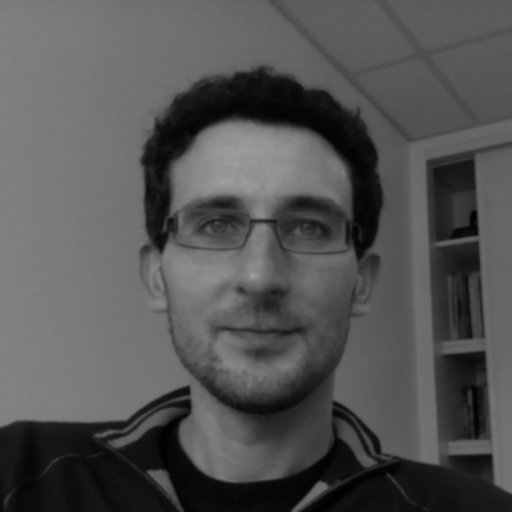
\includegraphics[width=1.75cm,height=1.75cm]{imgs/Cedric.jpg}}%
      \hspace*{0.3cm}
      \fbox{
\includegraphics[width=1.75cm,height=1.75cm]{imgs/Ayse.jpg}}
      \hspace*{0.3cm}
      \fbox{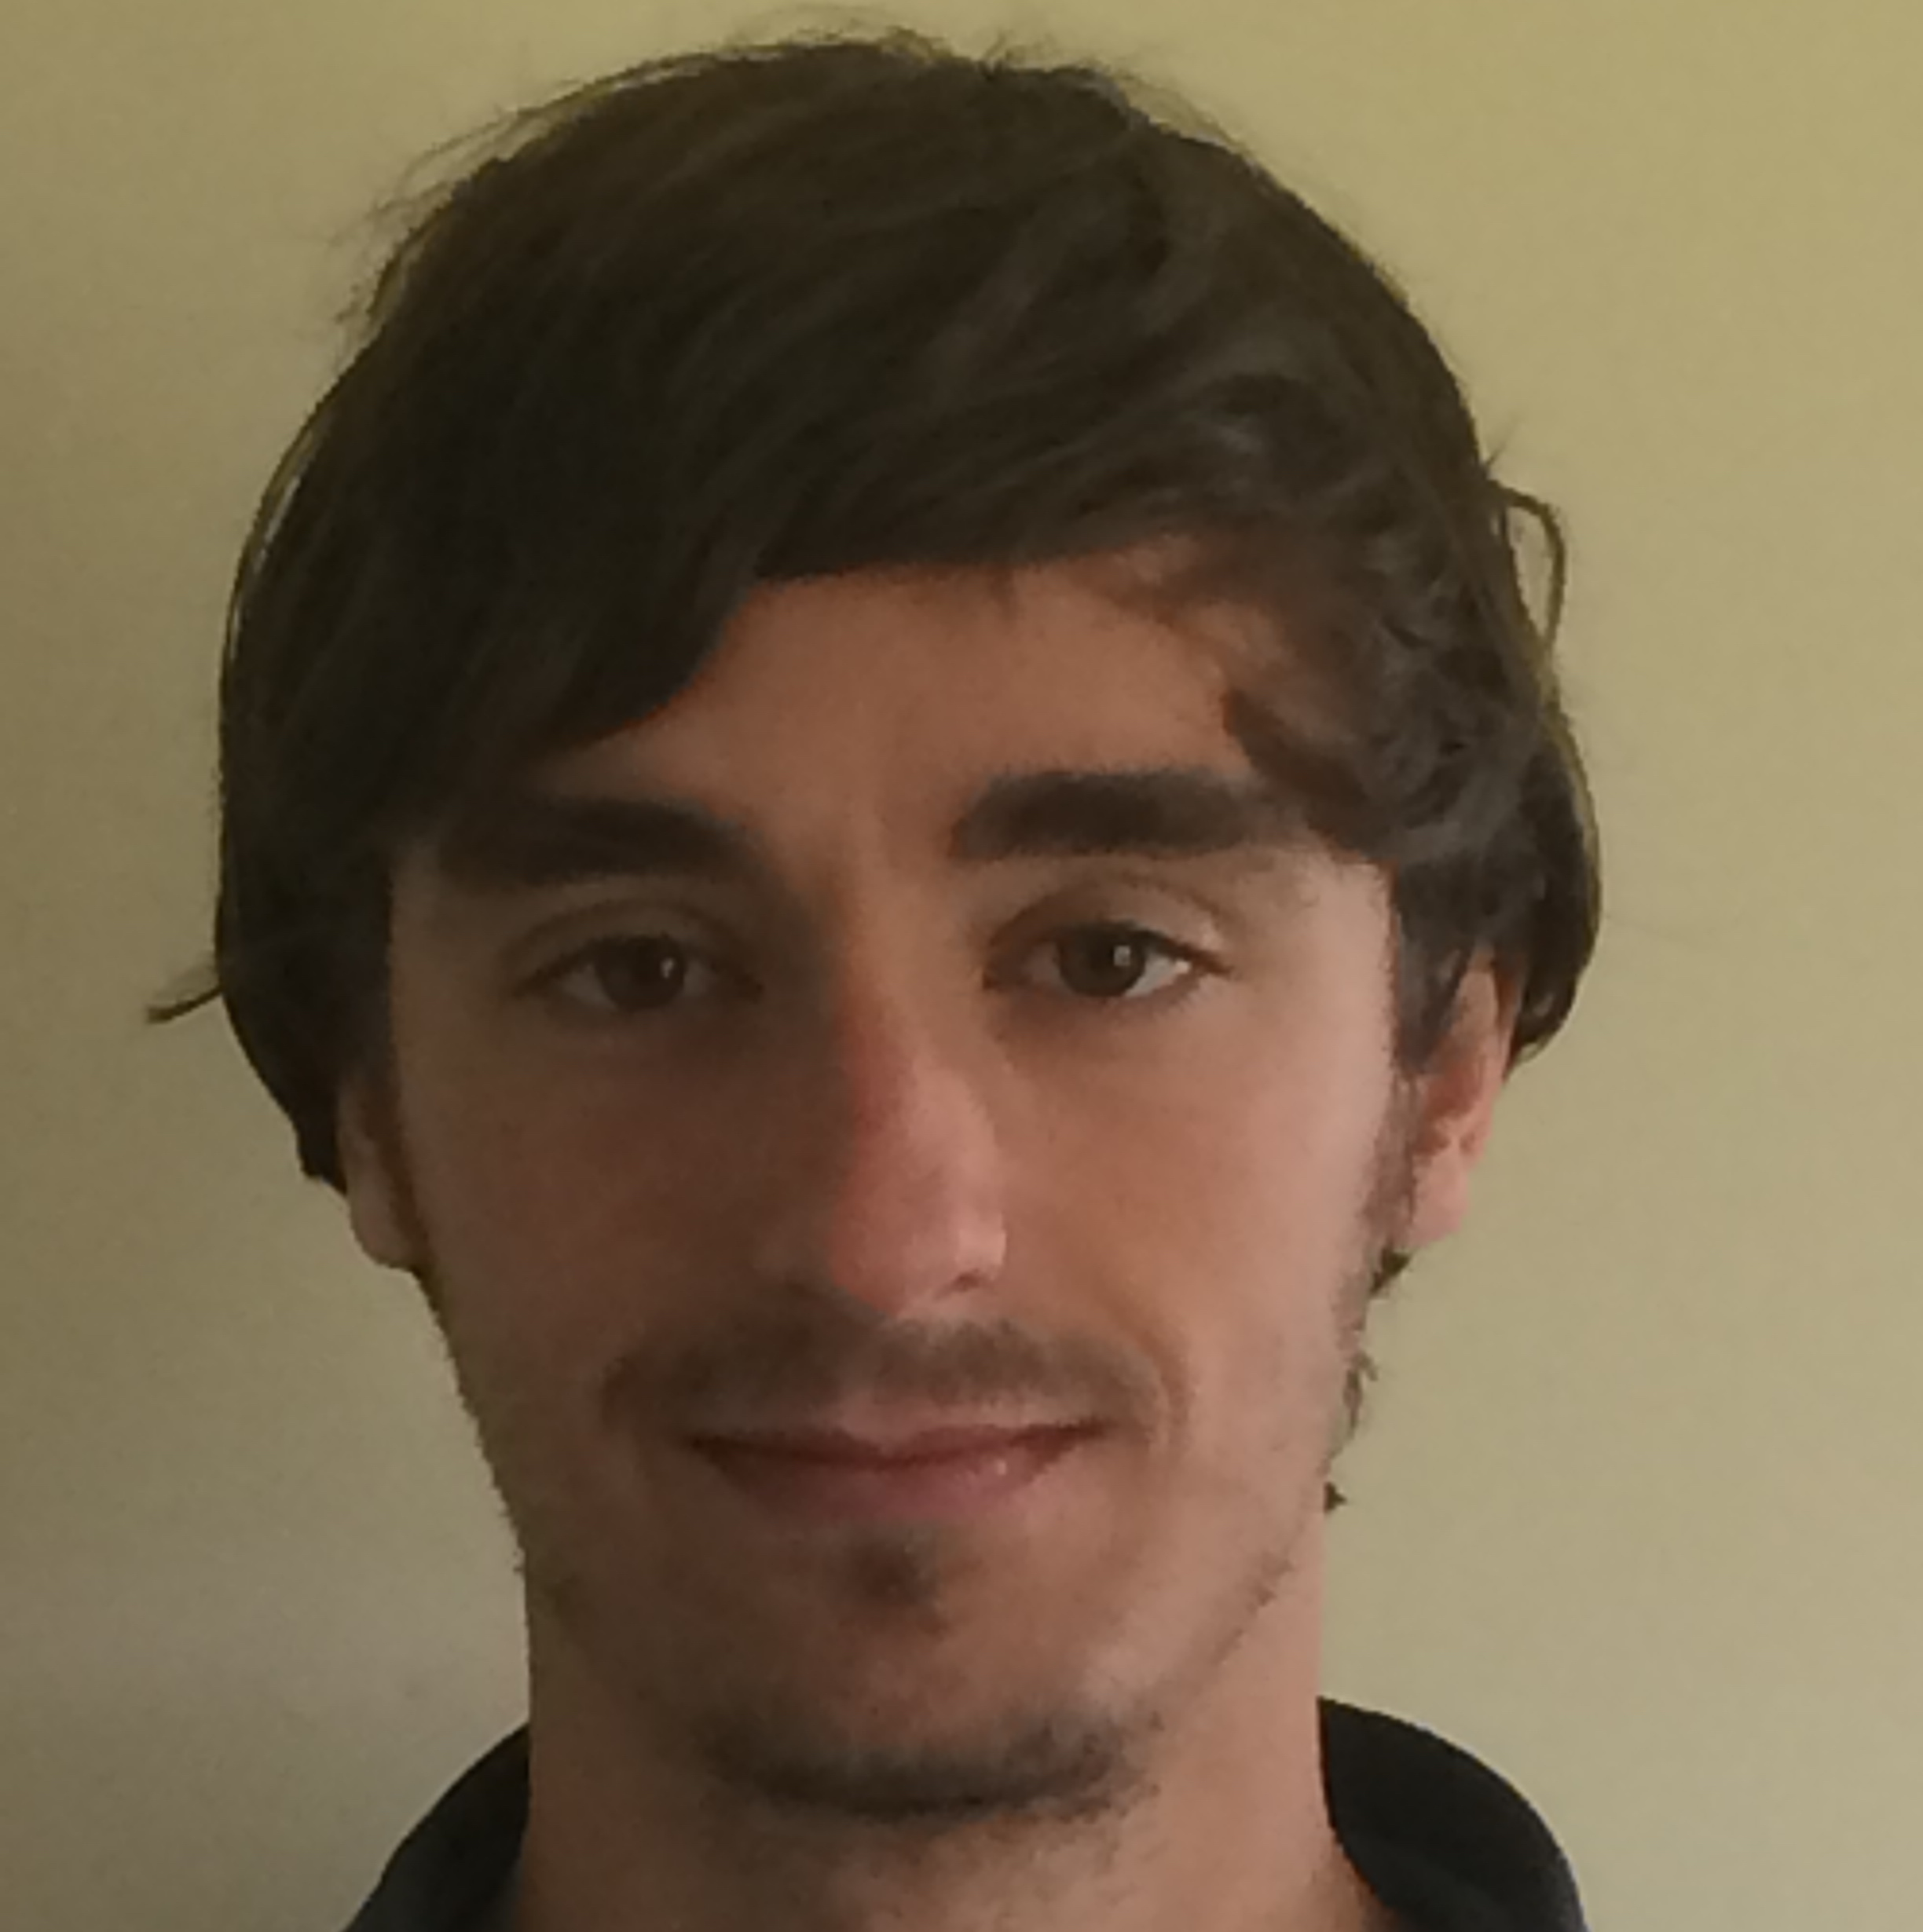
\includegraphics[width=1.75cm,height=1.75cm]{imgs/Clem.jpg}}
    }%
  }
}


\begin{document}

\maketitle

\begin{frame}{L0-penalized problems}
    \begin{tikzpicture}[remember picture,overlay,decoration={snake,amplitude=.4mm,segment length=2mm,post length=1mm}]
        \onslide<+-> {
            \draw [ultra thick,<->] ($(current page.north)+(-2.2,-0.32\textheight)$) -- ($(current page.north)+(2.2,-0.32\textheight)$) node (arrow) [midway] {};
            \node at ($(arrow.north)+(0,0.1)$) {\textbf{Objectives}};
        }
        %
        %
        %
        \node<+-> [text width=0.3\textwidth] at ($(current page.north)+(-4,-0.3\textheight)$) (obs) {
        \begin{blockone}{}
            \centering
            \textbf{Minimize a loss}
        \end{blockone}
        };
        %
        %
        %
        \node<+->[text width=.3\textwidth] at ($(current page.north)+(4,-0.3\textheight)$) (dic) {
        \begin{blocktwo}{}
            \centering
            \textbf{Sparse solution}
        \end{blocktwo}
        };
        %
        %
        %
        \node<+-> at ($(arrow.south)+(0,-0.6)$) (applications) {
            \begin{varwidth}{\linewidth}
                \centering
                \scriptsize{Machine Learning} \\
                \scriptsize{Signal processing} \\
                \scriptsize{Network design} \\
                \scriptsize{...}
            \end{varwidth}
        };
        %
        %
        %
        \node<+-> [text width=.45\textwidth] at ($(current page.north)+(0,-0.6\textheight)$) (problem) {
            \begin{blockthree}{$\ell_0$-penalized problem}
                \centering
                $\min_{\pv} \ \datafunc(\dic\pv) + \reg \norm{\pv}{0} + \regfunc(\pv)$
            \end{blockthree}
        };
    \end{tikzpicture}
    \begin{textblock}{1}(0.45,0.11)
        \begin{itemize}[nosep]
            \item[%
                \only<6->{$\datafunc(\dic\pv)$}%
            ]<6->: loss
            \item[$\norm{\pv}{0}$]<7-> : sparsity
            \item[$\reg$]<8-> : trade-off
            \item[$\regfunc(\pv)$]<9-> : modelling
        \end{itemize}
    \end{textblock}
\end{frame}
\begin{frame}{Contributions}
    \begin{tikzpicture}[remember picture,overlay]
        \node<+-> [text width=.45\textwidth] at ($(current page.north)+(0,-0.25\textheight)$) (problem) {
            \begin{blockthree}{$\ell_0$-penalized problem}
            \centering
            $\min_{\pv} \ \datafunc(\dic\pv) + \reg \norm{\pv}{0} + \regfunc(\pv)$
            \end{blockthree}
        };
        \node<+-> at ($(problem.south)+(0,-0.2)$) (problem) {
            \textbf{NP-hard}
        };
        \node<+-> [text width=.3\textwidth, anchor=north] at ($(problem.south)+(-4.1,-0.4)$) (mip) {
            \begin{blockzero}{Generic approach}
            \centering
            \scriptsize
            ~\\
            \begin{itemize}[leftmargin=*,label=$\blacktriangleright$,nosep]
                \item D. Bertsimas \hfill (2016)
                \item S. Bourguignon \hfill (2017)
                \item A. Atamtürk \hfill (2020)
                \item D. Bertsimas \hfill (2021)
                \item C. Kanzow \hfill (2022)
            \end{itemize}
            ~\\
            \onslide<+->{
                \emphone{
                \begin{itemize}[leftmargin=*,label=\ding{51},nosep]
                    \item MIP formulation
                \end{itemize}
                }
            }
            \onslide<+->{
                \emphone{
                \begin{itemize}[leftmargin=*,label=\ding{51},nosep]
                    \item Off-the-shelf solvers
                \end{itemize}
                }
            }
            \onslide<+->{
                \emphone{
                \begin{itemize}[leftmargin=*,label=\ding{51},nosep]
                    \item User friendly
                \end{itemize}
                }
            }
            \onslide<+->{
                \emphtwo{
                \begin{itemize}[leftmargin=*,label=\ding{55},nosep]
                    \item Slow
                \end{itemize}
                }
            }
            \end{blockzero}
        };
        \node<+-> [text width=.3\textwidth, anchor=north] at ($(problem.south)+(-0.1,-0.4)$) (bnb) {
            \begin{blockzero}{Tailored approach}
            \centering
            \scriptsize
            ~\\
            \begin{itemize}[leftmargin=*,label=$\blacktriangleright$,nosep]
                \item R. Ben Mhenni \hfill (2021)
                \item H. Hazimeh \hfill (2021)
                \item G. Samain \hfill (2022)
                \item A. Olama \hfill (2022)
                \item A. Atamtürk \hfill (2022)
            \end{itemize}
            ~\\
            \onslide<+->{
                \emphone{
                \begin{itemize}[leftmargin=*,label=\ding{51},nosep]
                    \item BnB algorithm
                \end{itemize}
                }
            }
            \onslide<+->{
                \emphone{
                \begin{itemize}[leftmargin=*,label=\ding{51},nosep]
                    \item Efficient bounding
                \end{itemize}
                }
            }
            \onslide<+->{
                \emphtwo{
                \begin{itemize}[leftmargin=*,label=\ding{55},nosep]
                    \item Restrictions on $\datafunc$ and $\regfunc$
                \end{itemize}
                }
            }
            \onslide<+->{
                \emphtwo{
                \begin{itemize}[leftmargin=*,label=\ding{55},nosep]
                    \item Inappropriate exploration
                \end{itemize}
                }
            }
            \end{blockzero}
        };
        \node<+-> [text width=.32\textwidth, anchor=north] at ($(problem.south)+(4,-0.4)$) (contrib) {
            \begin{blockzero}{Contributions}
            \centering
            \scriptsize
            ~\\
            \begin{itemize}[leftmargin=*,label=$\blacktriangleright$,nosep]
                \item This talk \hfill (2023)
                \item Extended paper \hfill (202?)
            \end{itemize}
            \begin{itemize}[leftmargin=*,nosep]
                \item 
                \item 
                \item 
            \end{itemize}
            ~\\
            \onslide<+->{
                \emphone{
                \begin{itemize}[leftmargin=*,label=\ding{51},nosep]
                    \item BnB algorithm
                \end{itemize}
                }
            }
            \onslide<+->{
                \emphone{
                \begin{itemize}[leftmargin=*,label=\ding{51},nosep]
                    \item Efficient bounding
                \end{itemize}
                }
            }
            \onslide<+->{
                \emphone{
                \begin{itemize}[leftmargin=*,label=\ding{51},nosep]
                    \item Generalize w.r.t. $\datafunc$ and $\regfunc$
                \end{itemize}
                }
            }
            \onslide<+->{
                \emphone{
                \begin{itemize}[leftmargin=*,label=\ding{51},nosep] 
                    \item Tailored exploration
                \end{itemize}
                }
            }
            \end{blockzero}
        };
    \end{tikzpicture}
\end{frame}
  
\begin{frame}{Branch-and-Bound}
    \begin{tikzpicture}[remember picture,overlay,decoration={snake,amplitude=.4mm,segment length=2mm,post length=1mm},domain=0:4]
        \node<+-> at (0,0) {};
        \onslide<+-> {
            \node [circle,draw=black,thick,top color = white,
            bottom color = blue!30,] at ($(current page.north)+(-3,-0.4\textheight)$) (node0) {$\nodeSymbIter{0}$};
        }
        %
        %
        %
        \onslide<+-> {
            \node [text width=.35\textwidth] at ($(node0.north)+(0,0.6)$) (problem) {
            \begin{blockthree}{}
                \centering
                \scriptsize
                $\min_{\pv} \ \datafunc(\dic\pv) + \reg \norm{\pv}{0} + \regfunc(\pv)$
            \end{blockthree}
            };
        }
        %
        %
        %
        \onslide<+-> {
            \node [circle,draw=black,thick,top color = white,
            bottom color = blue!30,] at ($(node0.south)+(-1.5,-1)$) (node1) {$\nodeSymbIter{1}$};
            \node [circle,draw=black,thick,top color = white,
            bottom color = blue!30,] at ($(node0.south)+(+1.5,-1)$) (node2) {$\nodeSymbIter{2}$};
            \draw [thick,->] (node0.south west) -- (node1.north east) node (arrow01) [midway] {};
            \draw [thick,->] (node0.south east) -- (node2.north west) node (arrow02) [midway] {};
        }
        %
        %
        %
        \onslide<+-> {
            \node at (arrow01) [fill=white,draw=black,thick] {\scriptsize{$\pvi{1} = 0$}};
            \node at (arrow02) [fill=white,draw=black,thick] {\scriptsize{$\pvi{1} \neq 0$}};
        }
        %
        %
        %
        \onslide<+> {
            \node [text width=.2\textwidth] at ($(node1.south)+(0,-0.6)$) (subprob1) {
                \begin{blockthree}{}
                    \scriptsize
                    $ \ \min_{\pv} \ \text{Same obj.}$ \\
                    $ \ \ \text{s.t.} \ \ \pvi{1} = 0$
                \end{blockthree}
            };
            \node [text width=.2\textwidth] at ($(node2.south)+(0,-0.6)$) (subprob2) {
                \begin{blockthree}{}
                    \scriptsize
                    $ \ \min_{\pv} \ \text{Same obj.}$ \\
                    $ \ \ \text{s.t.} \ \ \pvi{1} \neq 0$
                \end{blockthree}
            };
        }
        %
        %
        %
        \onslide<+-> {
            \node [circle,draw=black,thick,top color = white,
            bottom color = blue!30,] at ($(node1.south)+(-0.75,-1.25)$) (node3) {$\nodeSymbIter{3}$};
            \node [circle,draw=black,thick,top color = white,
            bottom color = blue!30,] at ($(node1.south)+(+0.75,-1.25)$) (node4) {$\nodeSymbIter{4}$};
            \node [circle,draw=black,thick,top color = white,
            bottom color = blue!30,] at ($(node2.south)+(-0.75,-1.25)$) (node5) {$\nodeSymbIter{5}$};
            \node [circle,draw=black,thick,top color = white,
            bottom color = blue!30,] at ($(node2.south)+(+0.75,-1.25)$) (node6) {$\nodeSymbIter{6}$};
            \draw [thick,->] (node1.south west) -- (node3.north) node (arrow13) [fill=white,draw=black,midway] {\scriptsize{$\pvi{2} = 0$}};
            \draw [thick,->] (node1.south east) -- (node4.north) node (arrow14) [fill=white,draw=black,midway] {\scriptsize{$\pvi{2} \neq 0$}};
            \draw [thick,->] (node2.south west) -- (node5.north) node (arrow25) [fill=white,draw=black,midway] {\scriptsize{$\pvi{2} = 0$}};
            \draw [thick,->,black] (node2.south east) -- (node6.north) node (arrow26) [fill=white,draw=black,midway] {\scriptsize{$\pvi{2} \neq 0$}};
        }
        %
        %
        %
        \onslide<+-> {
            \node [circle,draw=black,thick,top color = white,
            bottom color = blue!30,] at ($(current page.north)+(3,-0.4\textheight)$) (node) {$\nodeSymbIter{k}$};
            \draw [thick,->] ($(node.north)+(0,0.3)$) -- (node.north) {};
            \node at ($(node.south)+(0,-0.4)$) (subprob) {\small\textbf{Subproblem}};
            \node at ($(subprob.south)+(0,-0.1)$) (nphard) {\small{Still NP-hard}};
        }
        %
        %
        %
        \onslide<+-> {
            \node at ($(nphard.south)+(-1.5,-0.75)$) (heur) {\small\textbf{Heuristic}};
            \draw [thick,->,decorate] (nphard.south west) -- (heur.north) {};
            \node at ($(heur.south)+(0,-0.1)$) (upperbound) {\small{Upper bound}};
        }
        %
        %
        %
        \onslide<+-> {
            \node at ($(nphard.south)+(1.5,-0.75)$) (relax) {\small\textbf{Relaxation}};
            \draw [thick,->,decorate] (nphard.south east) -- (relax.north) {};
            \node at ($(relax.south)+(0,-0.1)$) (lowerbound) {\small{Lower bound}};
        }
        %
        %
        %
        \onslide<+-> {
            \node at ($(nphard.south)+(0,-2)$)  (pruning) {\small\textbf{Pruning rule}};
            \draw [thick,->,decorate] (upperbound.south) -- (pruning.north west) {};
            \draw [thick,->,decorate] (lowerbound.south) -- (pruning.north east) {};
        }
        %
        %
        %
        \onslide<+-> {
            \node at ($(pruning.south)+(0,-0.1)$) (rule) {\small{Node LB > Best UB}};
        }
        %
        %
        %
        \onslide<+-> {
            \node at ($(node4.south)+(0,-0.125)$) (bullet4) {$\bullet$};
            \draw [thick] (node4.south) -- ($(bullet4.south)+(0,0.2)$);
            \node at ($(node5.south)+(0,-0.125)$) (bullet5) {$\bullet$};
            \draw [thick] (node5.south) -- ($(bullet5.south)+(0,0.2)$);
            \node at ($(node6.south)+(0,-0.125)$) (bullet6) {$\bullet$};
            \draw [thick] (node6.south) -- ($(bullet6.south)+(0,0.2)$);
        }
        \onslide<+-> {
            \draw [thick,->] (node3.south west) -- ($(node3.south west)+(-0.1,-0.2)$);
            \draw [thick,->] (node3.south east) -- ($(node3.south east)+(0.1,-0.2)$);
        }
    \end{tikzpicture}
\end{frame}
\begin{frame}{Structural bottleneck}
    \setbeamercovered{
        again covered={\opaqueness<1->{10}}
    }
    \begin{tikzpicture}[remember picture,overlay,decoration={snake,amplitude=.4mm,segment length=2mm,post length=1mm},domain=0:4]
        \node<+-> at (0,0) {};
        \onslide<+-> {
            \node [circle,draw=black,thick,top color = white,
            bottom color = blue!30,] at ($(current page.north)+(-2,-0.25\textheight)$) (node0) {$\nodeSymbIter{0}$};
        }
        %
        %
        %
        \onslide<+-26> {
            \node [circle,draw=black,thick,top color = white,
            bottom color = blue!30,] at ($(node0.south)+(0.75,-1.25)$) (node1) {$\nodeSymbIter{1}$};
            \draw [thick,->] (node0.south east) -- (node1.north) node (arrow01) [fill=white,draw=black,midway] {\scriptsize{$\pvi{1} \neq 0$}};
        }
        %
        %
        %
        \onslide<+-26> {
            \node at ($(node1.south)+(0,-0.125)$) (bullet1) {$\bullet$};
            \draw [thick] (node1.south) -- ($(bullet1.south)+(0,0.2)$);
        }
        %
        %
        %
        \onslide<+-26> {
            \node [circle,draw=black,thick,top color = white,
            bottom color = blue!30,] at ($(node0.south)+(-0.75,-1.25)$) (node2) {$\nodeSymbIter{2}$};
            \draw [thick,->] (node0.south west) -- (node2.north) node (arrow02) [fill=white,draw=black,midway] {\scriptsize{$\pvi{1} = 0$}};
        }
        %
        %
        %
        \uncover<+-26> {
            \node [circle,draw=black,thick,top color = white,
            bottom color = blue!30,] at ($(node2.south)+(0.75,-1.25)$) (node3) {$\nodeSymbIter{3}$};
            \draw [thick,->] (node2.south east) -- (node3.north) node (arrow23) [fill=white,draw=black,midway] {\scriptsize{$\pvi{2} \neq 0$}};
        }
        %
        %
        %
        \onslide<+-26> {
            \node at ($(node3.south)+(0,-0.125)$) (bullet3) {$\bullet$};
            \draw [thick] (node3.south) -- ($(bullet3.south)+(0,0.2)$);
        }
        %
        %
        %
        \onslide<+-26> {
            \node [circle,draw=black,thick,top color = white,
            bottom color = blue!30,] at ($(node2.south)+(-0.75,-1.25)$) (node4) {$\nodeSymbIter{4}$};
            \draw [thick,->] (node2.south west) -- (node4.north) node (arrow23) [fill=white,draw=black,midway] {\scriptsize{$\pvi{2} = 0$}};
        }
        %
        %
        %
        \onslide<+-26> {
            \node [circle,draw=black,thick,top color = white,
            bottom color = blue!30,] at ($(node4.south)+(0.75,-1.25)$) (node5) {$\nodeSymbIter{5}$};
            \draw [thick,->] (node4.south east) -- (node5.north) node (arrow35) [fill=white,draw=black,midway] {\scriptsize{$\pvi{3} \neq 0$}};
        }
        %
        %
        %
        \onslide<+-26> {
            \node at ($(node5.south)+(0,-0.125)$) (bullet5) {$\bullet$};
            \draw [thick] (node5.south) -- ($(bullet5.south)+(0,0.2)$);
        }
        %
        %
        %
        \onslide<+-> {
            \node [circle,draw=black,thick,top color = white,
            bottom color = blue!30,] at ($(node4.south)+(-0.75,-1.25)$) (node6) {$\nodeSymbIter{6}$};
            \draw [thick,->] (node6.south west) -- ($(node6.south west)+(-0.1,-0.2)$);
            \draw [thick,->] (node6.south east) -- ($(node6.south east)+(0.1,-0.2)$);
        }
        \onslide<11-26> {
            \draw [thick,->] (node4.south west) -- (node6.north) node (arrow36) [fill=white,draw=black,midway] {\scriptsize{$\pvi{3} = 0$}};
        }
        %
        %
        %
        \only<12-> {
            \node [text width=0.15\textwidth] at ($(node5.south)+(0.25,-0.75)$) (goodbranch) {
                \begin{blocktwo}{}
                    \centering
                    \scriptsize{Always pruned}
                \end{blocktwo}
            };
        }
        %
        %
        %
        \only<13-> {
            \node [text width=0.15\textwidth] at ($(node6.south)+(-0.25,-0.75)$) (goodbranch) {
                \begin{blocktwo}{}
                    \centering
                    \scriptsize{No bound improvment}
                \end{blocktwo}
            };
        }
        %
        %
        %
        \node<+-> at(0,0) {};
        \node<+-> at (0,0) {};
        \onslide<+-> {
            \node [text width=0.5\textwidth] at ($(current page.north)+(3,-2.5)$) (waste) {
                \small
                \begin{blocksix}{}
                    \centering
                    \small
                    \textbf{Waste of computational power !}
                \end{blocksix}
            };
        }
        %
        %
        %
        \onslide<+-> {
            \node [text width=0.5\textwidth] at ($(waste.south)+(0,-0.75)$) (question) {
                \small
                \begin{blocksix}{}
                    \centering
                    \small
                    \textbf{How to avoid such situations ?}
                \end{blocksix}
            };
            \draw [ultra thick,->] ($(waste.south)+(0,0)$) -- ($(question.north)+(0,-0.3)$);
        }
        %
        %
        %
        \onslide<+-> {
            \node [text width=0.5\textwidth] at ($(question.south)+(0,-0.75)$) (answer) {
                \begin{blocksix}{}
                    \centering
                    \small
                    \textbf{Leverage duality link between nodes}
                \end{blocksix}
            };
            \draw [ultra thick,->] ($(question.south)+(0,0)$) -- ($(answer.north)+(0,-0.3)$);
        }
        %
        %
        %
        \onslide<+-> {
            \node [circle,draw=black,thick,top color = white,
            bottom color = blue!30,] at ($(answer.south)+(-1.5,-0.5)$) (nodek) {$\nodeSymbIter{0}$};
            \node [circle,draw=black,thick,top color = white,
            bottom color = blue!30,] at ($(answer.south)+(1.5,-0.5)$) (nodekp) {$\nodeSymbIter{1}$};
            \draw [thick,->] (nodek.east) -- (nodekp.west);
        }
        %
        %
        %
        \onslide<+-> {
            \node at ($(nodek.south)+(0,-0.25)$) (nodeksub) {\scriptsize{Subproblem}};
            \node at ($(nodekp.south)+(0,-0.25)$) (nodekpsub) {\scriptsize{Subproblem}};
        }
        %
        %
        %
        \onslide<+-> {
            \node at ($(nodeksub.south)+(0,-0.25)$) (nodekrelax) {\scriptsize{Relaxation}};
            \node at ($(nodekpsub.south)+(0,-0.25)$) (nodekprelax) {\scriptsize{Relaxation}};
            \draw [thick,->] ($(nodekpsub.south)+(0,0.05)$) -- ($(nodekprelax.north)+(0,-0.05)$);
            \draw [thick,->] ($(nodeksub.south)+(0,0.05)$) -- ($(nodekrelax.north)+(0,-0.05)$);
        }
        %
        %
        %
        \onslide<+-> {
            \node at ($(nodekrelax.south)+(0,-0.25)$) (nodekdual) {\scriptsize{\emphtwo{Dual}}};
            \draw [thick,->,color=mLightBrown] ($(nodekrelax.south)+(0,0.05)$) -- ($(nodekdual.north)+(0,-0.05)$);
            \node at ($(nodekprelax.south)+(0,-0.25)$) (nodekpdual) {\scriptsize{\emphtwo{Dual}}};
            \draw [thick,->,color=mLightBrown] ($(nodekprelax.south)+(0,0.05)$) -- ($(nodekpdual.north)+(0,-0.05)$);
        }
        %
        %
        %
        \onslide<+-> {
            \draw [thick,<->,color=mLightBrown,dashed] ($(nodekdual.east)+(0.05,0)$) -- ($(nodekpdual.west)+(-0.05,0)$) node [midway] (link) {};
        }
        %
        %
        %
        \onslide<+-> {
            \node at ($(nodekdual.south)+(0,-0.15)$) (dual1) {\scriptsize{\emphtwo{$\max_{\dv} \dfunc(\dv)$}}};
        }
        %
        %
        %
        \onslide<+-> {
            \node at ($(nodekpdual.south)+(0,-0.15)$) (dual1) {\scriptsize{\emphtwo{$\max_{\dv} \dfunc(\dv) + r(u)$}}};
        }
        %
        %
        %
        \onslide<+-> {
            \node at ($(dual1.south)+(-0.5,-0.5)$) (complexity) {\scriptsize\emphtwo{$\mathcal{O}(1)$}};
            \draw[mLightBrown,thick,->] (complexity.east) .. controls ($(dual1.south)+(0.6,-0.45)$) .. ($(dual1.south)+(0.75,0)$);
        }
        %
        %
        %
        \onslide<+-> {
            \draw[mLightBrown,ultra thick,->] (node0.west) .. controls ($(node0.west)+(-2.2,-0.25)$) .. ($(node0.north west)+(-2.5,-1.75)$);
            \node[draw=mLightBrown,thick,top color = white,bottom color = orange!25,font=\scriptsize,align=center,ultra thick] at ($(node0.north west)+(-2.5,-1.75)$) (fix1) {Fix $\pvi{1} = 0$ \\ Fix $\pvi{2} = 0$ \\ Fix $\pvi{3} = 0$ };
        }
        %
        %
        %
        \onslide<+-> {
            \draw[mLightBrown,ultra thick,->] (fix1.south) .. controls ($(fix1.south)+(0,-2)$) .. (node6.north west);
        }
        %
        %
        %
        \node<+-> at (0,0) {};
        %
        %
        %
        \onslide<+-> {
            \node [text width=0.25\textwidth] at ($(current page.center)+(-2.2,1)$) (effect1) {
                \small
                \begin{blockone}{}
                    \centering
                    \scriptsize
                    \textbf{Avoid useless nodes}
                \end{blockone}
            };
        }
        %
        %
        %
        \onslide<+-> {
            \node [text width=0.25\textwidth] at ($(effect1.south)+(0,-0.3)$) (effect2) {
                \small
                \begin{blockone}{}
                    \centering
                    \scriptsize
                    \textbf{Save computations}
                \end{blockone}
            };
        }
        %
        %
        %
        \onslide<+-> {
            \node [text width=0.25\textwidth] at ($(effect2.south)+(0,-0.3)$) (effect3) {
                \small
                \begin{blockone}{}
                    \centering
                    \scriptsize
                    \textbf{Reduce solving time}
                \end{blockone}
            };
        }
    \end{tikzpicture}
\end{frame}
\begin{frame}{Variable fixing}
    \begin{tikzpicture}[remember picture,overlay,decoration={snake,amplitude=.4mm,segment length=2mm,post length=1mm},domain=0:4]
        \node at ($(current page.north)+(-4.7,-8.7)$) (origin) {};
        \onslide<+-> {
            \node [circle,draw=black,thick,top color = white,
            bottom color = blue!30,] at ($(current page.north)+(0,-2)$) (node) {$\nodeSymbIter{k}$};
            \draw [thick,->] ($(node.north)+(0,0.3)$) -- (node.north);
        }
        %
        %
        %
        \onslide<+-> {
            \node [text width=0.3\textwidth] at ($(node.east)+(3,0.25)$) (objective) {
                \small
                \begin{blocksix}{}
                    \centering
                    \textbf{Identify an index $j$}
                \end{blocksix}
            };
        }
        %
        %
        %
        \onslide<+-> {
            \node [circle,draw=black,thick,top color = white,
            bottom color = blue!30,font=\small,dashed] at ($(node.south)+(1.25,-1)$) (node1) {$\nodeSymbIter{k}_{j}$};
            \node at ($(node1.south)+(0,-0.125)$) (bullet) {$\bullet$};
            \draw [thick] (node1.south) -- ($(bullet.south)+(0,0.2)$);
            \draw [thick,->,dashed] (node.south east) -- (node1.north west) node (arrow01) [fill=white,draw=black,midway] {\scriptsize{$\pvi{j} \neq 0$}};
        }
        %
        %
        %
        \onslide<+-> {
            \draw[mLightBrown,ultra thick,->] (node.north west) .. controls ($(node.north)+(-2.5,1)$) and ($(node.south)+(-2.5,-1)$) .. (node.south west);
            \node[draw=mLightBrown,thick,top color = white,bottom color = orange!25,font=\scriptsize,align=center,ultra thick] at ($(node.west)+(-1.5,0)$) (fix) {Fix $\pvi{j} = 0$};
        }
        %
        %
        %
        \onslide<+-> {
            \node[align=center] at ($(origin)+(2.5,3.8)$) {\small\textbf{Relaxation resolution at} $\nodeSymbIter{k}$};
            \draw[->,thick] ($(origin)+(-0.2,0)$) -- ($(origin)+(5,0)$) node[below left] {\scriptsize{iterations}};
            \draw[->,thick] ($(origin)+(0,-0.2)$) -- ($(origin)+(0,4)$) node[above] {};
            \node [text width=0.4\textwidth] at ($(current page.north)+(3.5,-6.5)$) (ingredients) {
                \small
                \begin{blocksix}{Ingredients}
                \begin{itemize}[leftmargin=*,label=$\bullet$,nosep]
                    \item<7-> Already-computed quantities
                    \item<8-> Cost-free dual evaluation
                    \item<10-> Dual link between nodes
                    \item<14-> Can fix \textbf{multiple} variables
                \end{itemize} 
                \end{blocksix}
            };
        }
        %
        %
        %
        \onslide<+-> {
            \node[font=\scriptsize,align=center] at ($(origin)+(-0.8,3.3)$) (fix1) {\textcolor{blue!50}{Relax. obj.} \\ \textcolor{blue!50}{at node $N^k$}};
            \begin{scope}[shift={(0.22,-2.2)},scale=0.5]
                \draw [color=blue!50,domain=1:10,samples=200,variable=\x,thick] plot (\x,{5*(sin(20*\x r)/(10*\x^2))+exp(-0.8*\x+2)});
            \end{scope}
        }
        %
        %
        %
        \node<+-> at (0,0) {};
        \node<+-> at (0,0) {};
        %
        %
        %
        \onslide<+-> {
            \node[font=\scriptsize,align=center] at ($(origin)+(-0.8,0.3)$) (fix1) {\textcolor{blue!50}{Dual. obj.} \\ \textcolor{blue!50}{at node $N^k$}};
            \begin{scope}[shift={(0.22,-2.2)},scale=0.5]
                \draw [color=blue!50,domain=1:10,samples=200,variable=\x,thick] plot (\x,{-5*(sin(20*\x r)/(10*\x^2))-exp(-1.5*\x+2)});
            \end{scope}
        }
        %
        %
        %
        \node<+-> at (0,0) {};
        %
        %
        %
        \onslide<+-> {
            \node[font=\scriptsize,align=center] at ($(origin)+(-0.8,1.15)$) {\textcolor{blue!50}{Dual obj.} \\ \textcolor{blue!50}{at node $N^k_{j}$}};
            \begin{scope}[shift={(0.22,-2)},scale=0.5]
                \draw [color=blue!50,domain=1:10,samples=200,variable=\x,thick,dashed] plot (\x,{-5*(sin(10*\x r)/(10*\x^2))-exp(-0.8*\x+2)+2});
            \end{scope}
        }
        %
        %
        %
        \onslide<+-> {
            \node at ($(origin)+(-0.7,2.35)$) {\scriptsize\textcolor{red!50}{Best UB}};
            \begin{scope}[shift={(0.22,-1.7)},scale=0.5]
                \draw [domain=1:10,samples=200,variable=\x,thick,color=red!50] plot (\x,0.9);
            \end{scope}
        }
        %
        %
        %
        \onslide<+-> {
            \draw[dashed,thick] ($(origin)+(1.25,2.3)$) -- ($(origin)+(1.25,0)$) {};
            \node at ($(origin)+(1.25,-0.25)$) {\scriptsize\textbf{Prune $N^k_{j}$}};
        }
        %
        %
        %
        \node<+-> at (0,0) {};
    \end{tikzpicture}
\end{frame}
\begin{frame}{Numerical illustrations}
  \begin{tikzpicture}[remember picture,overlay]
    \onslide {
      \node [text width=.45\textwidth] at ($(current page.north)+(0,-0.175\textheight)$) (problem) {
      \begin{blockthree}{}
          \centering
          \small
          $\min_{\pv} \ \datafunc(\dic\pv) + \reg \norm{\pv}{0} + \regfunc(\pv)$
      \end{blockthree}
      };
    }
    %
    %
    %
    \node<+-> [text width=.7\textwidth] at ($(current page.north)+(2,-0.325\textheight)$) (data) {
      \begin{itemize}[nosep]
        \item<+->[\textbf{Dataset}] : Sparse linear regression
        \item<+->[\textbf{F(Ax)}] : Mean squared error
        \item<+->[\textbf{G(x)}] : Constraint $\boldsymbol{l} \leq \boldsymbol{x} \leq \boldsymbol{u}$
      \end{itemize}
    };
    \onslide<+-> {
      \begin{scope}[shift={(1,-2.5)}]
        \begin{axis}[
          mlineplot,
          width=0.8\textwidth,
          height=5cm,
          xmode=log,
          log basis x={10},
          ymax = 110,
          yticklabel={\pgfmathprintnumber\tick\,\%},
          xlabel = Time (seconds),
          ylabel = Instances solved,
          legend style={at={(1.03,0.5)},anchor=west}
        ]
          
          \addplot[ultra thick,color=RoyalBlue4,visible on=<6->] %
          table[x=times,y=DirectSolver-scip,col sep=comma]{data/synthetic_optimize_LeastSquares_BigmL2norm_10_250_500_0.1_32.0.csv};
          \only<6-> {
            \addlegendentry{SCIP};
          }

          \addplot[ultra thick,color=SteelBlue2,visible on=<6->] %
          table[x=times,y=DirectSolver-cplex,col sep=comma]{data/synthetic_optimize_LeastSquares_BigmL2norm_10_250_500_0.1_32.0.csv};
          \only<6-> {
            \addlegendentry{CPLEX};
          }

          \addplot[ultra thick,color=SkyBlue1,visible on=<6->] %
          table[x=times,y=DirectSolver-mosek,col sep=comma]{data/synthetic_optimize_LeastSquares_BigmL2norm_10_250_500_0.1_32.0.csv};
          \only<6-> {
            \addlegendentry{MOSEK};
          }

          \addplot[ultra thick,color=LightSalmon1,visible on=<7->] %
          table[x=times,y=BourguignonSolver,col sep=comma]{data/synthetic_optimize_LeastSquares_BigmL2norm_10_250_500_0.1_32.0.csv};
          \only<7-> {
            \addlegendentry{Bourguignon \hfill(2022)};
          }

          \addplot[ultra thick,color=LightPink3,visible on=<7->] %
          table[x=times,y=HazimehSolver,col sep=comma]{data/synthetic_optimize_LeastSquares_BigmL2norm_10_250_500_0.1_32.0.csv};
          \only<7-> {
            \addlegendentry{Hazimeh (2022)};
          }

          \addplot[ultra thick,color=Brown4,visible on=<8->] %
          table[x=times,y=BnbSolver-accel,col sep=comma]{data/synthetic_optimize_LeastSquares_BigmL2norm_10_250_500_0.1_32.0.csv};
          \only<8-> {
            \addlegendentry{\textbf{Proposed}};
          }
        \end{axis}
      \end{scope}
    }
  \end{tikzpicture}
\end{frame}
\begin{frame}{Numerical illustrations}
    \begin{tikzpicture}[remember picture,overlay]
        \node<+-> [text width=0.8\textwidth] at ($(current page.north)+(0,-0.3\textwidth)$) (highlights) {
            \begin{block}{Highlights}
                \begin{itemize}[label=$\bullet$]
                    \item<+-> Gains up to $\times10^5$ against MIP solvers 
                    \item<+-> Gains up to $\times10^2$ against tailored BnB 
                    \item<+-> Scales up to dimension $\approx 10^5$ in minutes
                \end{itemize}
            \end{block}
        };
        \onslide<+-> {
            \draw[ultra thick] (0.22\textwidth,-0.23\textheight) rectangle (0.78\textwidth,-0.05\textheight);
            \node [text width=0.7\textwidth] at ($(current page.north)+(0,-0.55\textwidth)$) (repo) {
                \begin{textblock}{1}(0.1,-0.025)
                    \LARGE{TheoGuyard/\bf{El0ps.jl}}
                \end{textblock}
                \begin{textblock}{1}(0.11,0.055)
                    \scriptsize{\textcolor{gray}{An Exact L0-penalized Problem Solver.}}
                \end{textblock}
                \begin{textblock}{1}(0.55,0.075)
                    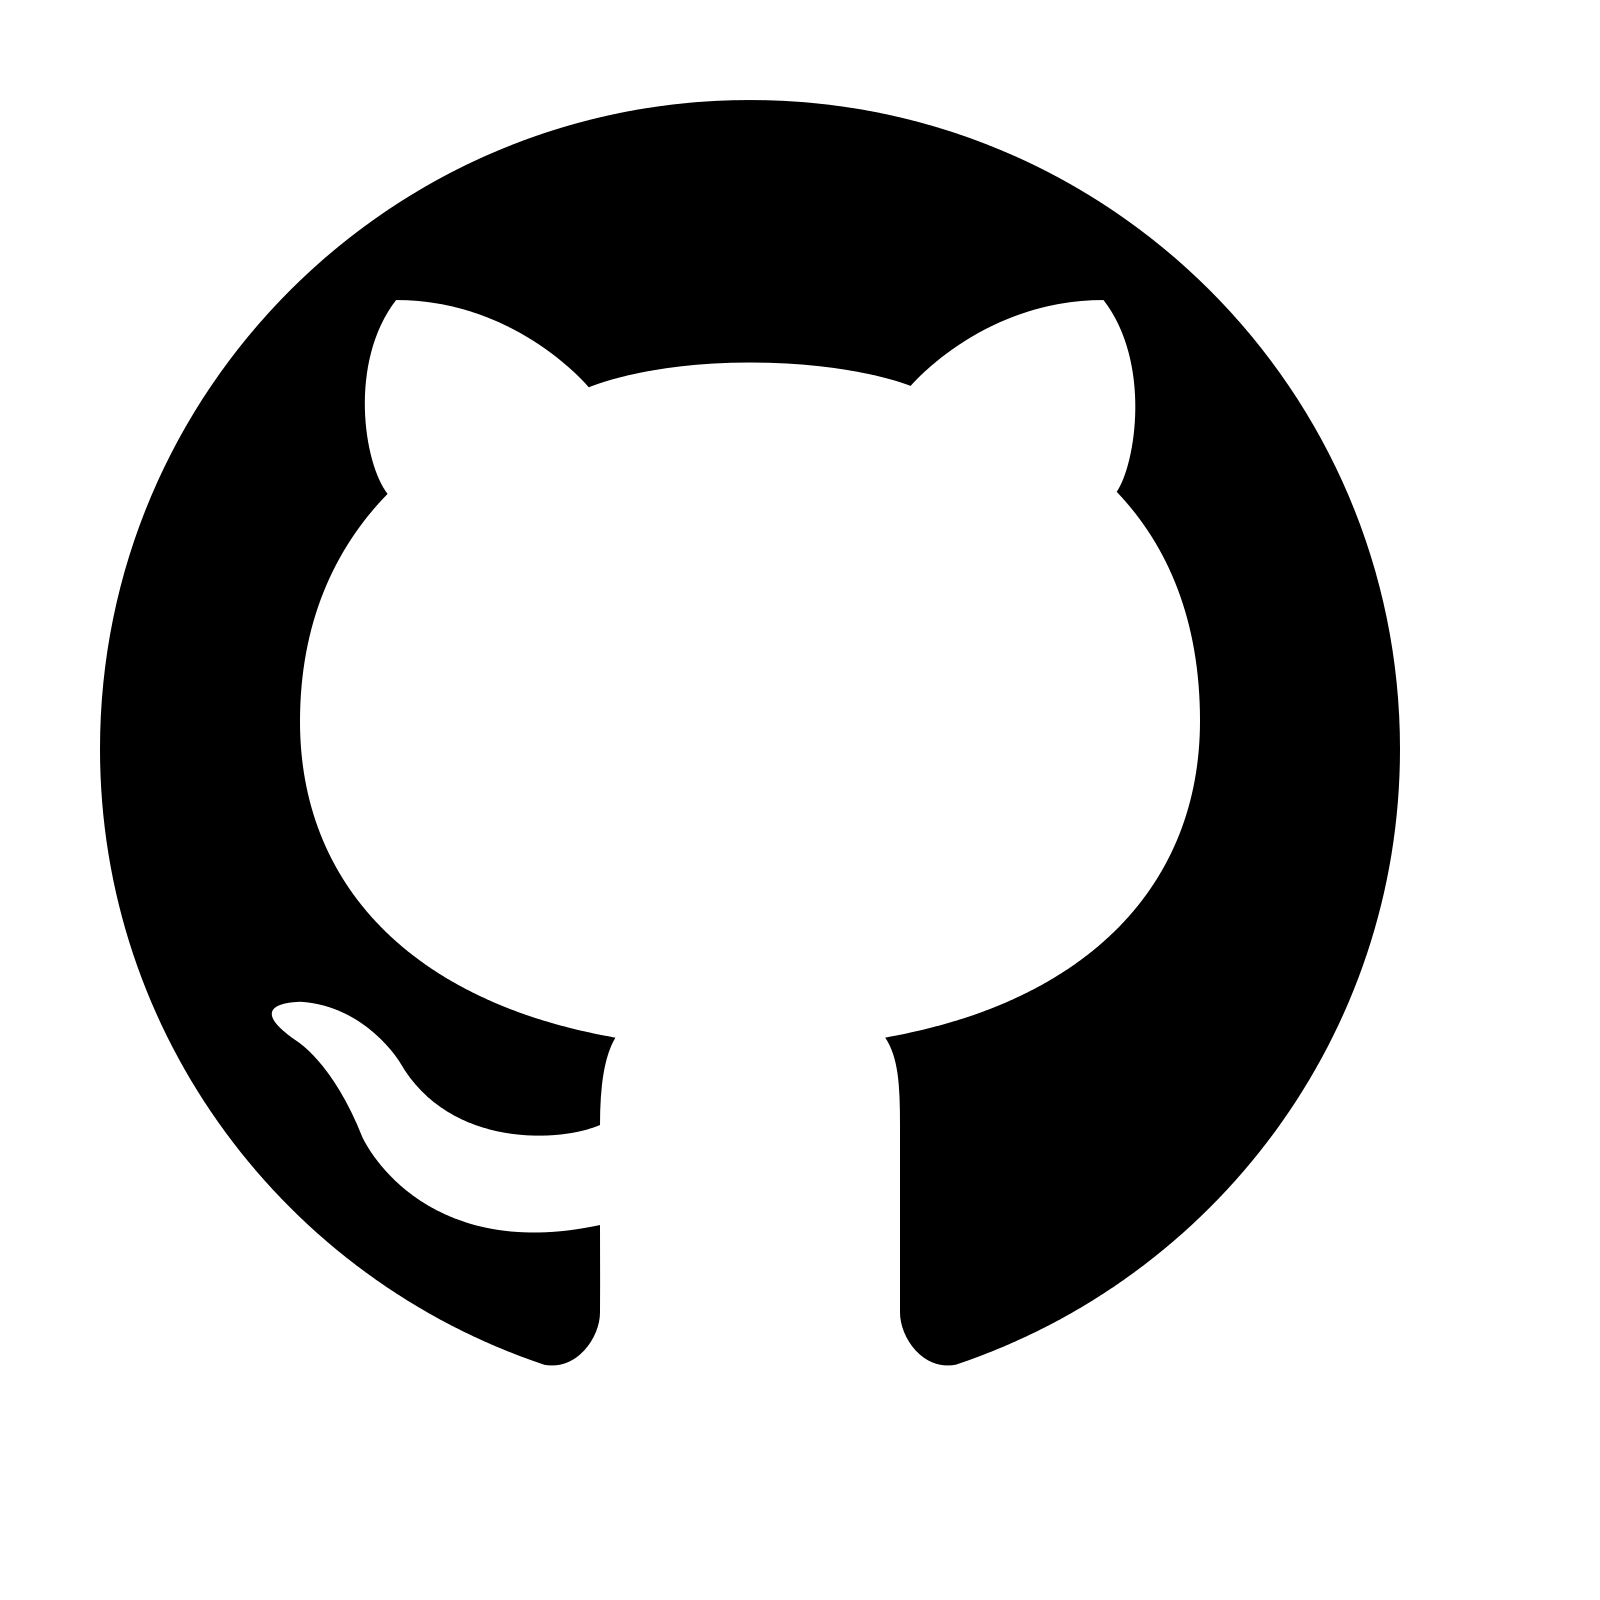
\includegraphics[width=0.04\textwidth]{imgs/github.png}
                \end{textblock}
            };
        }
        \onslide<+-> {
            \node [text width=0.3\textwidth, align=center] at ($(current page.north)+(-4,-0.47\textwidth)$) (efficient) {
                \small{Efficient BnB}
            };
            \draw[thick,->] (efficient.south) .. controls ($(efficient.south)+(0,-0.5)$) .. ($(efficient.south)+(0.75,-1)$);
            \node [text width=0.3\textwidth, align=center] at ($(efficient.south)+(-0.2,-0.7)$) (efficientimg) {
                
\includegraphics[width=15pt]{imgs/strong.png}
            };
        }
        \onslide<+-> {
            \node [text width=0.3\textwidth, align=center] at ($(current page.north)+(4,-0.47\textwidth)$) (generic) {
                \small{Generic framework}
            };
            \draw[thick,->] (generic.south) .. controls ($(generic.south)+(0,-0.5)$) .. ($(generic.south)+(-0.75,-1)$);
            \node [text width=0.3\textwidth, align=center,xscale=-1] at ($(generic.south)+(0.25,-0.75)$) (genericimg) {
                
\includegraphics[width=15pt]{imgs/strong.png}
            };
        }
        \onslide<+-> {
            \node [align=center] at ($(current page.north)+(0,-0.8\textwidth)$) (ggeneric) {
                \small{Works with any $\datafunc$ and $\regfunc$} \\ 
                \small{under mild assumptions !}
            };
            \draw[thick,->] (ggeneric.north) .. controls ($(ggeneric.north)+(0,0.5)$) .. ($(ggeneric.north)+(0,0.8)$);
            \node [text width=0.3\textwidth, align=center] at ($(ggeneric.north)+(0.6,0.4)$) (ggenericimg) {
                
\includegraphics[width=15pt]{imgs/party.png}
            };
        }
    \end{tikzpicture}
\end{frame}
\begin{frame}[standout]
    Question time !
\end{frame}

\begin{frame}[noframenumbering]{Working hypotheses}
    \begin{tikzpicture}[remember picture,overlay,domain=-0.8:0.8]
        \node [text width=.7\textwidth] at ($(current page.north)+(0,-0.275\textheight)$) (datafunc) {
            \begin{blocksix}{Loss function}
                \small
                Assumptions on $\datafunc$ :
                \begin{itemize}[label=$\bullet$,nosep]
                    \item $\datafunc$ is proper, convex, lower-semicontinuous
                    \item $\datafunc$ is differentiable with $\grad\datafunc$ being $\lipschitz$-Lipschitz
                \end{itemize}
            \end{blocksix}
        };
        \node [text width=.7\textwidth] at ($(datafunc.south)+(0,-0.15\textheight)$) (regfunc) {
            \begin{blocksix}{Modelling term}
                \small
                Assumptions on $\regfunc$ :
                \begin{itemize}[label=$\bullet$,nosep]
                    \item $\regfunc$ is proper, convex, lower-semicontinuous
                    \item $\regfunc = \sum_{\idxentry} \separable{\regfunc}{\idxentry}$ with $\separable{\regfunc}{\idxentry} \geq \separable{\regfunc}{\idxentry}(0) = 0$
                \end{itemize}
            \end{blocksix}
        };
        \node (origin) at ($(current page.south)+(0,1)$) {};
        \draw[->] ($(origin)+(-2,0)$) -- ($(origin)+(2,0)$);
        \draw[->] ($(origin)+(0,-0.1)$) -- ($(origin)+(0,2)$);
        \node[right] at ($(origin)+(2,0)$) {$\pv$};
        \draw[teal,thick] ($(origin)+(-1.8,1.5)$) .. controls ($(origin)+(0,-0.5)$) .. ($(origin)+(1.8,1.5)$);
        \node at ($(origin)+(2,1.1)$) (norms) {\scriptsize\textcolor{teal}{Norms}};
        \draw[mLightBrown,thick] ($(origin)+(-1.3,0)$) -- ($(origin)+(1.3,0)$);
        \draw[mLightBrown,thick,dashed] ($(origin)+(-1.3,1.8)$) -- ($(origin)+(-1.3,0)$);
        \draw[mLightBrown,thick,dashed] ($(origin)+(1.3,0)$) -- ($(origin)+(1.3,1.8)$);
        \draw[mLightBrown,thick] ($(origin)+(1.3,1.8)$) -- ($(origin)+(1.9,1.8)$);
        \draw[mLightBrown,thick] ($(origin)+(-1.3,1.8)$) -- ($(origin)+(-1.9,1.8)$);
        \node at ($(origin)+(2.2,1.8)$) {\scriptsize\emphtwo{$+\infty$}};
        \node at ($(origin)+(1.3,-0.3)$) {\scriptsize\emphtwo{Constr. fulfilled at $\pv = 0$}};
    \end{tikzpicture}
\end{frame}
\begin{frame}[noframenumbering]{Node problems}
    \begin{tikzpicture}[remember picture,overlay]
        \node [circle,draw=black,thick,top color = white,
        bottom color = blue!30,] at ($(current page.north)+(-4,-0.2\textheight)$) (node) {$\nodeSymbIter{k}$};
        \node[align=left] at ($(node.south)+(0,-0.8)$) (node-fixing) {
            \small{$\setzero = \kset{\idxentry}{\pvi{\idxentry} = 0}$} \\ 
            \small{$\setone = \kset{\idxentry}{\pvi{\idxentry} \neq 0}$} \\ 
            \small{$\setnone = \kset{\idxentry}{\pvi{\idxentry} \ \text{free}}$}
        };
        \node [text width=.7\textwidth] at ($(current page.north)+(1.6,-0.275\textheight)$) (subproblem) {
            \begin{blockthree}{Subproblem}
                \small
                $$
                \left\{
                \begin{array}{rl}
                    \min_{\pv} & \ \datafunc(\dic\pv) + \reg \norm{\pv}{0} + \regfunc(\pv) \\
                    \text{s.t.} & \ \subzero{\pv} = \0, \ \subone{\pv} \neq \0
                \end{array}
                \right.
                $$
                NP-hard unless $\setnone = \emptyset$.
            \end{blockthree}
        };
        \node [text width=\textwidth,anchor=north] at ($(current page.north)+(0,-0.45\textheight)$) (relaxation) {
            \begin{blocktwo}{Relaxation}
                \small
                $$
                \textstyle\min_{\pv} \big\{ \datafunc(\dic\pv) + \relaxregfunc(\pv) \big\}
                $$
                with $\relaxregfunc(\pv)$ being the convex envelope of  $\reg \norm{\pv}{0} + \regfunc(\pv) + \Icvx(\subzero{\pv}=\0,\subone{\pv}\neq\0)$.
            \end{blocktwo}
        };
        \node [text width=\textwidth,anchor=north] at ($(relaxation.south)+(0,-0.01\textheight)$) (dual) {
            \begin{blockone}{Dual}
                \small
                $$
                \textstyle\max_{\dv} \big\{ -\conj{\datafunc}(-\dv) - \conj{\relaxregfunc}(\transp{\dic}\dv) \big\}
                $$
                with $\conj{\relaxregfunc}(\transp{\dic}\dv)= \textstyle\sum_{\idxentry \in \setnone} \pospart{\conj{\regfunc}(\transp{\atom{\idxentry}}\dv) - 1} + \textstyle\sum_{\idxentry \in \setone} (\conj{\regfunc}(\transp{\atom{\idxentry}}\dv) - 1)$
            \end{blockone}
        };
    \end{tikzpicture}
\end{frame}



\end{document}